% ==============================================================================
%  Pure Black-Box Uncertainty Quantification via Distilled Proxies
%  ACL-format paper. Requires the official ACL style files in this directory:
%    acl.sty, acl_natbib.bst   (from https://github.com/acl-org/acl-style-files)
%  Compile:  pdflatex main ; bibtex main ; pdflatex main ; pdflatex main
%  If acl.sty is unavailable, the FALLBACK block below reproduces a close layout
%  with stock packages (comment out \usepackage[review]{acl} and uncomment the fallback).
% ==============================================================================
\documentclass[11pt]{article}

\usepackage[review]{acl}                 % <-- official ACL style
% ---------- FALLBACK (uncomment if acl.sty is missing) ----------
% \usepackage[margin=1in]{geometry}
% \usepackage{natbib}
% \bibliographystyle{plainnat}
% ----------------------------------------------------------------

\usepackage{times}
\usepackage{latexsym}
\usepackage[T1]{fontenc}
\usepackage[utf8]{inputenc}
\usepackage{microtype}
\usepackage{booktabs}
\usepackage{amsmath}
\usepackage{amssymb}
\usepackage{multirow}
\usepackage{graphicx}
\usepackage{xcolor}
\usepackage{url}
\usepackage{enumitem}
\usepackage{pgfplots}
\pgfplotsset{compat=1.17}
\usepgfplotslibrary{groupplots}

\newcommand{\ours}{\textsc{Ours}}
\newcommand{\dald}{\textsc{DALD}}
\newcommand{\disaad}{\textsc{DisAAD}}
\newcommand{\ppl}{\textsc{Ppl}}
\newcommand{\best}[1]{\textbf{#1}}

\title{Read-Out, Not Objective: A Latency-First Benchmark of \\
Pure Black-Box Uncertainty Quantification with Distilled Proxies}

% author block omitted: [review] mode emits "Anonymous ACL submission".
% CAMERA-READY: restore \author{...} here.
\begin{document}
\maketitle

\begin{abstract}
Deployed language-model systems increasingly call \emph{black-box} targets whose logits and
weights are inaccessible, yet still need a fast signal for \emph{when the target is wrong}. We
study \emph{distilled-proxy} uncertainty quantification: a small white-box student is distilled
from the target's \emph{text} alone, and its logits are read out at near-constant,
target-decoupled latency. Within one controlled harness we compare three proxy
\emph{objectives}---masked SFT (\dald), adversarial SFT (\disaad), and an uncertainty-aware
variant (\ours)---across two open teachers, six students, and seven task domains, holding the
base model, distillation data, and evaluation fixed. Our central finding is negative and
actionable: \textbf{the read-out dominates the training objective}. Holding the proxy fixed, the
choice of logit read-out moves AUROC by $0.107$--$0.109$, while the objectives span only
$0.011$--$0.028$ at any fixed read-out---a $4$--$10\times$ gap---so we find no evidence the
objectives differ at deployable operating points. Which read-out wins is itself
teacher-dependent, so the claim concerns the axis, not an estimator. Three leave-one-dataset-out
refutations further show that \emph{any} scheme fitting a combination across domains fails to
transfer, making the per-dataset ``oracle ceiling'' unreachable. What survives is a clear
recommendation: one proxy, one fixed read-out, no routing, at $24$--$44$\,ms---a
$250$--$790\times$ latency reduction for a $0.02$--$0.09$ AUROC price.
\end{abstract}

% ==============================================================================
\section{Introduction}
% ==============================================================================
Large language models (LLMs) are frequently deployed as \emph{black boxes}: an
application calls a hosted API or a served endpoint and receives only \emph{text}.
Provider policies, tokenizer mismatches, and serving stacks routinely hide the
target's log-probabilities, hidden states, and weights. Yet the downstream system
still needs to know \emph{when to trust an answer}---to abstain, escalate, or defer.
This is the pure black-box UQ setting: estimate the probability that a target's answer
is incorrect \emph{using its text output only}.

The dominant black-box UQ methods---sampling-based semantic consistency
\citep{kuhn2023semantic,farquhar2024detecting,lin2024generating} and verbalized
self-confidence \citep{lin2022teaching}---share a structural cost: they pay for
\emph{additional target generations} (several samples, or a self-report call). On a
70B model or a frontier API this is seconds to tens of seconds per item, which is
often larger than the original answer's latency budget. A promising alternative
\emph{decouples} the UQ cost from the target entirely: distill a small \emph{white-box}
proxy from the target's text, and read the proxy's own logits. The proxy is trained
once; at inference it performs a single small forward pass, so its latency is a
near-constant floor independent of the target's size or price.

Three published training objectives instantiate this idea.
\dald~\citep{zeng2024dald} distills a surrogate by masked supervised fine-tuning
(SFT) on the target's outputs so that logit-based detectors align.
\disaad (Distribution-Aligned Adversarial Distillation)~\citep{cui2026disaad} adds a
discriminator-based adversarial regularizer to align the surrogate's output distribution
with the target's and reads uncertainty via an evidential (Dirichlet) head. A natural
third variant, which we call \ours, adds an
\emph{uncertainty-aware} distillation term that supervises the proxy's evidential
uncertainty toward a black-box oracle computed on the teacher's samples. Prior work
reports these methods with their \emph{native} read-outs and on their native tasks,
which makes cross-method comparison confounded: differences in reported AUROC may
reflect the read-out or the task rather than the objective.

We build a single controlled benchmark that isolates the objective---same base model,
same distillation data, same evaluation, same save format---and ask a sequence of
increasingly skeptical questions.\footnote{Code, configurations, and analysis scripts:
\url{[repository URL withheld for anonymous review]}} Our contributions are:

\begin{enumerate}[leftmargin=1.4em,itemsep=1pt,topsep=2pt]
\item \textbf{A latency-first, pure black-box UQ benchmark} (\S\ref{sec:setup})
spanning two open teachers, six students, three proxy objectives, nine logit
read-outs, and seven task domains, with target-relative latency as a first-class axis.
\item \textbf{The read-out $\gg$ objective finding} (\S\ref{sec:readout}): on
non-degenerate cells the nine read-outs span $0.107$--$0.109$ AUROC on the same proxy, while
the three objectives span $0.011$--$0.028$ at a fixed read-out. The best read-out is
teacher-dependent---perplexity on Qwen (by $0.003$, within noise), evidential EDL-AU on
Llama---so we claim the axis, not an estimator. Once read-out is controlled we cannot
separate the objectives.
\item \textbf{Three LODO refutations of combination} (\S\ref{sec:combiners}): a
score-level stacker, per-dataset configuration selection, and a
domain$\rightarrow$read-out router (the deployable core of a proxy mixture-of-experts)
each \emph{fail to transfer out-of-sample}, worse than a single fixed choice. The
per-dataset oracle ceiling is therefore a mirage, not a target.
\item \textbf{A grey-box comparison} (\S\ref{sec:greybox}) showing the black-box proxy
loses essentially nothing to reading the target's own logits---except the specific
\emph{P(True)} probe---and a mechanistic account of \emph{why} (cross-perplexity beats
contaminated self-perplexity).
\item \textbf{A deployable recommendation} (\S\ref{sec:discussion}): one proxy,
one fixed read-out, no routing, at $\sim$25--45\,ms; reserve target-coupled verbalized
confidence for safety-critical queries where it clearly dominates.
\end{enumerate}

We regard the negative results as the paper's most useful output. They are cheap to
state and expensive to rediscover, and they sharpen what a proxy UQ system should and
should not attempt.

% ==============================================================================
\section{Related Work}
% ==============================================================================
\paragraph{Black-box UQ for LLMs.} When logits are unavailable, uncertainty is
typically read from \emph{sampled text}. Semantic entropy clusters multiple samples by
bidirectional entailment and measures dispersion
\citep{kuhn2023semantic,farquhar2024detecting}; graph-spectral variants
(eccentricity, degree, eigenvalue scores) summarize the same similarity graph
\citep{lin2024generating}. These are strong but pay for $N$ target generations.
\emph{Verbalized confidence} elicits a self-reported score in one extra call
\citep{lin2022teaching}, and \emph{P(True)} reads the target's probability of the token
``true'' \citep{kadavath2022language}---the latter requires target log-probabilities and
is therefore \emph{grey-box}, which we treat as an upper comparison rather than a
pure-BB method.

\paragraph{White-box logit estimators.} On a model whose logits are visible, one can
read maximum softmax probability \citep{hendrycks2017baseline}, predictive entropy,
energy scores \citep{liu2020energy}, evidential/Dirichlet uncertainty
\citep{sensoy2018evidential,malinin2021uncertainty}, and length-normalized sequence
likelihood (perplexity). Our proxies are white-box \emph{by construction}, so all of
these apply to the proxy's logits without ever touching the target.

\paragraph{Distilled surrogates.} \dald~\citep{zeng2024dald} aligns a small surrogate
to a black-box model by SFT on its generations, enabling curvature detectors
\citep{bao2024fastdetectgpt} for machine-text detection. \disaad~\citep{cui2026disaad}
adds an adversarial objective for hallucination detection. We reproduce both objectives
faithfully and add an uncertainty-aware term (\ours), then \emph{repurpose the family}
as pure black-box \emph{correctness} estimators---distinct from the original
text-detection goal. Our library builds on \textsc{TruthTorchLM}
\citep{bakman2024truthtorchlm}.

\paragraph{Mixtures and routing.} Combining specialists via a gate is classical
\citep{jacobs1991moe}. We test the score-level and read-out-level cores of such a
combiner and find they do not survive leave-one-dataset-out, which bears directly on
whether a proxy mixture-of-experts is worth building.

% ==============================================================================
\section{Benchmark and Setup}\label{sec:setup}
% ==============================================================================
\paragraph{Pipeline.} We follow a four-axis design $G\times D\to M\to V$: generator
(target) $G$, dataset $D$, method $M$, metric $V$. For each $(G,D)$ we generate and
\emph{cache} the target's answers once; every method and every sample budget reads the
same cache, guaranteeing a fair comparison and preventing wasted generation. Labels use
an LLM judge (MCQ match for multiple-choice). The metric is AUROC of the uncertainty
score against answer incorrectness, with AUPRC, ECE, and a latency frontier as
secondary. \emph{Pure black-box} is enforced at the interface: methods see the target's
text only; the proxy's whiteness comes from distillation on that text, never from the
target's internals.

\paragraph{Targets and students.} Open teachers are Qwen3-32B \citep{yang2024qwen3} and
Llama-3.3-70B \citep{dubey2024llama3}; we also report a closed arm (GPT-4o,
Claude-Haiku-4.5) accessed through a text-only gateway. Students span Qwen3
$\{0.6,1.7,4\}$B and Llama-3.2/3.1 $\{1,3,8\}$B. Proxies are LoRA adapters
\citep{hu2022lora} (rank 32, $\alpha{=}64$) on the seven attention/MLP projections. The
two \emph{best-student} cells used throughout the results are Qwen3-32B$\to$qwen3-4b and
Llama-3.3-70B$\to$llama3.2-3b.

\paragraph{Objectives.} All three share the base, the LoRA configuration, and the
distillation set (a fixed 400-prompt mixture); they differ \emph{only} in the training
loss:
\[
\begin{aligned}
\dald  &: \; \mathcal{L}_{\text{task}} \quad(\text{masked distillation, response tokens only})\\
\disaad&: \; \mathcal{L}_{\text{task}} + \lambda_{\text{adv}}\,\mathcal{L}_{\text{reg}}\\
\ours  &: \; \mathcal{L}_{\text{task}} + \lambda_{\text{adv}}\,\mathcal{L}_{\text{reg}} + \lambda\,\mathcal{L}_{\text{unc}}
\end{aligned}
\]
Following \disaad, $\mathcal{L}_{\text{task}}(\theta)=-\frac{1}{NM}\sum_{i,j}\sum_t\log
P_\theta(y_t\mid y_{<t})$ is the token-level distillation loss (prompt tokens masked) and
$\mathcal{L}_{\text{reg}}$ is the sequence-level adversarial regularizer against a
discriminator $\mathcal{M}_D$ (App.~\ref{app:readouts}). Our added term
$\mathcal{L}_{\text{unc}}$ pushes the proxy's top-$k$ Dirichlet evidential uncertainty
(or an MLP head) toward a black-box oracle $u^\star(x)\in[0,1]$ computed on the
teacher's samples (Eccentricity or Discrete Semantic Entropy). $\lambda$, the oracle,
and the read-out (\texttt{edl}/\texttt{head}) define the \ours\ variant grid.

\paragraph{Read-outs.} On any proxy's logits over the answer span we compute nine
estimators: evidential aleatoric/epistemic (EDL-AU/EU), maximum-softmax (MSP), entropy,
energy, LogTokU, and---new to this study---three \emph{likelihood} read-outs that use
which token the target actually emitted: \emph{perplexity} (mean negative
log-likelihood), \emph{MaxNLL} (weakest-token NLL), and \emph{LogitMargin}. The first
six read only distribution shape; the likelihood family reads the emitted token.

\paragraph{Datasets.} Seven, one per category, 150 items each: TriviaQA (General)
\citep{joshi2017triviaqa}, BioASQ (Medical, open) \citep{tsatsaronis2015bioasq}, MedQA
(Medical, MCQ) \citep{jin2021medqa}, MedLFQA (Medical, long-form), GSM8K (Math)
\citep{cobbe2021gsm8k}, TruthfulQA (Adversarial) \citep{lin2021truthfulqa}, and a
Wikipedia factual set (Factual). Cells are $127$--$150$ items after filtering.
\textbf{Class balance and exclusions.} Because AUROC is undefined without both classes and
unstable when one is tiny, we exclude any cell whose minority class is $<15$. This removes
BioASQ on the Llama teacher, which has a \emph{single} incorrect answer ($149/150$ correct),
and MedLFQA on Qwen ($139/150$). Both were included in an earlier version of this analysis and
materially changed the read-out ranking (\S\ref{sec:readout}); we report the corrected means
throughout and give per-cell counts in Appendix~\ref{app:details}.

\paragraph{Latency protocol.} Following the black-box premise, latency is measured
\emph{relative to the target}: batch size 1, GPU warm-up before timing, exclusive
allocation, median (p50) over items. The proxy read-out is a single small forward pass;
direct methods additionally pay the target's per-sample generation cost.

% ==============================================================================
\section{Results}\label{sec:results}
% ==============================================================================
We present the headline proxy comparison, then the read-out finding, the grey-box
ceiling, direct methods, and the domain analysis. All AUROC; the two best-student cells.

\subsection{Objectives tie at every deployable operating point}

Table~\ref{tab:triptych} reports each proxy under three disclosure tiers. The
\emph{ceiling} selects the best variant \emph{and} read-out per dataset using the test
labels---an oracle. \emph{Best-var} fixes one \ours\ configuration
(\texttt{head\_ecc}$\cdot$\ppl) chosen by overall mean. \emph{Deploy} fixes
\texttt{base}$\cdot$perplexity a priori.

\begin{table}[t]\centering\small
\setlength{\tabcolsep}{3.2pt}
\begin{tabular}{l ccc ccc}
\toprule
& \multicolumn{3}{c}{\textbf{Qwen3-32B}} & \multicolumn{3}{c}{\textbf{Llama-3.3-70B}}\\
\cmidrule(lr){2-4}\cmidrule(lr){5-7}
& ceil & best & \best{dep} & ceil & best & \best{dep}\\
\midrule
\ours   & 0.690 & 0.616 & 0.612 & 0.715 & 0.626 & 0.609\\
\dald   & 0.668 & 0.604 & 0.603 & 0.697 & \best{0.632} & \best{0.632}\\
\disaad & 0.675 & \best{0.613} & \best{0.613} & 0.683 & 0.611 & 0.611\\
\bottomrule
\end{tabular}
\caption{Proxy comparison, mean AUROC, three disclosure tiers (\S\ref{sec:results}).
At the (label-cheating) ceiling \ours\ leads by $\sim$0.02; the moment a single fixed
configuration is committed, the lead vanishes---Qwen ties to \disaad, Llama inverts to
\dald. \ours\ falls the most from ceiling to deploy ($-$0.08/$-$0.11) because its ceiling
leaned hardest on per-dataset cherry-picking.}
\label{tab:triptych}
\end{table}

The story is entirely in the collapse from \emph{ceil} to \emph{dep}. At the ceiling
\ours\ leads both teachers ($+0.02$). At any deployable setting the three objectives are
tied within noise, and \dald---the simplest, purely-SFT surrogate---is the nominal best
on Llama. The objective does not separate the methods.

Table~\ref{tab:perds} gives the per-dataset deployable view with measured latency. No
proxy owns a domain deployably; per-dataset winners are split across all three, and the
means are within $\pm0.02$.

\begin{table}[t]\centering\small
\setlength{\tabcolsep}{3pt}
\begin{tabular}{l ccc ccc}
\toprule
& \multicolumn{3}{c}{\textbf{Qwen}$\to$q4b} & \multicolumn{3}{c}{\textbf{Llama}$\to$l3b}\\
\cmidrule(lr){2-4}\cmidrule(lr){5-7}
dataset & \ours & \dald & \disaad & \ours & \dald & \disaad\\
\midrule
trivia (Gen)     & 0.623 & 0.605 & \best{0.634} & \best{0.664} & 0.631 & 0.647\\
bioasq (Med)     & --    & --    & --    & 0.987 & \best{0.993} & 0.987\\
medqa (MCQ)      & \best{0.713} & 0.578 & 0.690 & 0.528 & \best{0.600} & 0.452\\
medlfqa (Med-LF) & \best{0.526} & 0.519 & 0.500 & 0.448 & \best{0.450} & 0.444\\
gsm8k (Math)     & 0.773 & \best{0.854} & 0.781 & \best{0.696} & 0.694 & 0.693\\
truthful (Adv)   & 0.477 & \best{0.510} & 0.477 & \best{0.554} & 0.551 & 0.554\\
wiki (Fact)      & 0.585 & 0.560 & \best{0.598} & 0.506 & \best{0.507} & 0.499\\
\midrule
\textbf{MEAN}    & \best{0.616} & 0.604 & 0.613 & 0.626 & \best{0.632} & 0.611\\
\midrule
\multicolumn{7}{l}{\emph{latency p50 (ms), batch 1:}}\\
q4b: & 41.4 & 43.1 & 44.3 & \multicolumn{3}{l}{l3b: 24.1 / 31.9 / 34.1}\\
\bottomrule
\end{tabular}
\caption{Deployable per-dataset AUROC (single fixed config$\cdot$read-out) and measured
latency. Qwen \ours$=$\texttt{head\_ecc}$\cdot$\ppl; Llama all $\cdot$perplexity. Bioasq
is degenerate on Qwen (trivially separable) and omitted from its mean. Latency is
identical across objectives---one forward on the same student.}
\label{tab:perds}
\end{table}

\subsection{The read-out dominates the objective}\label{sec:readout}

Applying all nine estimators to the same proxy logits (Table~\ref{tab:readout}) shows that
the \emph{choice of read-out} is by far the larger lever. On non-degenerate cells the nine
read-outs span $0.107$ AUROC on Qwen ($0.523$--$0.630$) and $0.109$ on Llama
($0.467$--$0.577$), whereas the three training objectives, held at a fixed read-out, span only
$0.011$ and $0.028$. The read-out moves AUROC $4$--$10\times$ more than the objective---this,
not any particular estimator, is the paper's central claim.

\emph{Which} read-out wins is teacher-dependent, and we caution against the stronger claim.
On Qwen, perplexity leads at $0.630$, but only by $0.003$ over max-softmax---inside noise. On
Llama the evidential EDL-AU read-out leads at $0.577$, ahead of perplexity's $0.545$. An
earlier version of this analysis reported perplexity as the universal winner; that conclusion
depended on the BioASQ cell, which has a \emph{single} negative example on the Llama teacher
and is excluded here (\S\ref{sec:setup}). We report the corrected ranking and note the
methodological lesson: with $150$-item cells and skewed correctness, one degenerate dataset can
reverse a leaderboard.

\begin{table}[t]\centering\small
\begin{tabular}{l cc}
\toprule
read-out (on \ours-base) & Qwen & Llama\\
\midrule
EDL-AU (prior default)   & 0.523 & \best{0.577}\\
Entropy                  & 0.625 & 0.543\\
MSP                      & 0.627 & 0.545\\
Perplexity               & \best{0.630} & 0.545\\
MaxNLL                   & 0.566 & 0.548\\
LogTokU                  & 0.531 & 0.468\\
\bottomrule
\end{tabular}
\caption{Single read-out on the deployable proxy, mean AUROC over non-degenerate cells
(BioASQ excluded on Llama, MedLFQA on Qwen). The best read-out differs by teacher---perplexity
on Qwen (by $0.003$, within noise), EDL-AU on Llama---but the \emph{spread} across read-outs
($0.107$/$0.109$) dwarfs the spread across objectives ($0.011$/$0.028$). Read-out $\gg$
objective.}
\label{tab:readout}
\end{table}

The practical consequence is unchanged and is what we recommend: because no read-out wins
everywhere, and because the objectives are indistinguishable at any fixed read-out, the
deployable configuration is one proxy with one read-out chosen a priori---and the cost of
choosing wrongly among read-outs ($\sim$0.11) is an order of magnitude larger than the cost of
choosing the ``wrong'' objective ($\sim$0.01--0.03).

\subsection{Grey-box buys almost nothing---except P(True)}\label{sec:greybox}

Running the same nine read-outs on the \emph{target's own} logits (4-bit, grey-box
ceiling) yields a fair best-per-dataset \emph{lift over the black-box proxy of only}
$-0.011$ (Qwen) / $-0.014$ (Llama): the proxy's logits are as informative as the
target's. The sole grey-box method that beats the best proxy read-out is
\emph{P(True)} (0.662 / 0.659 vs perplexity 0.612 / 0.609, $\approx{+}0.05$). A
mechanism explains the near-parity: perplexity is \emph{weaker} on the target
(0.570/0.578) than on the proxy (0.612/0.609), because the target's \emph{self}-%
perplexity is contaminated---it generated the answer---whereas the proxy's
\emph{cross}-perplexity is a clean surprise signal. Cross-perplexity from a proxy is an
argument \emph{for} distillation, not merely a fallback.

\begin{figure}[t]
\centering
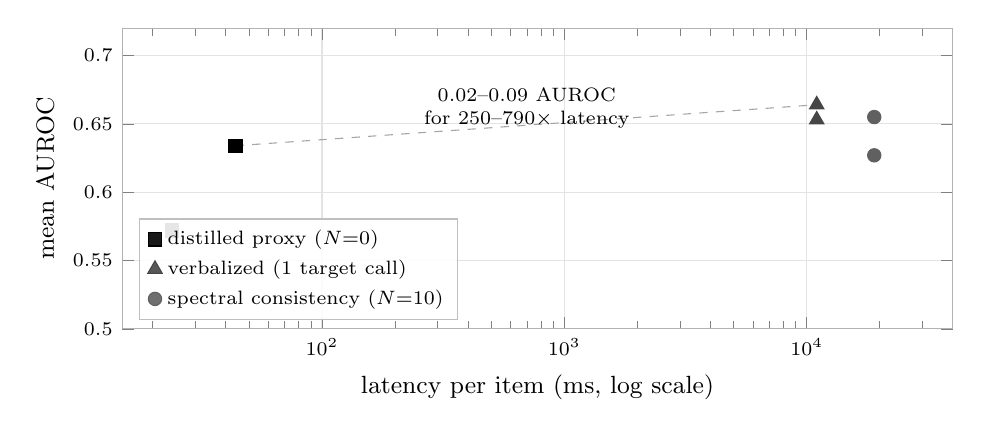
\begin{tikzpicture}
\begin{axis}[
  width=\columnwidth, height=5.4cm,
  xmode=log, log basis x=10,
  xlabel={latency per item (ms, log scale)},
  ylabel={mean AUROC},
  xmin=15, xmax=40000, ymin=0.50, ymax=0.72,
  xlabel style={font=\small}, ylabel style={font=\small},
  tick label style={font=\scriptsize},
  grid=major, grid style={gray!22}, axis line style={gray!60},
  legend style={font=\scriptsize, at={(0.02,0.03)}, anchor=south west,
                draw=gray!50, fill=white, fill opacity=0.9, text opacity=1},
  legend cell align=left,
]
% distilled proxies: target-decoupled, one small forward pass
\addplot[only marks, mark=square*, mark size=2.4pt, black] coordinates {(24,0.572) (44,0.634)};
\addlegendentry{distilled proxy ($N{=}0$)}
% verbalized confidence: one target call
\addplot[only marks, mark=triangle*, mark size=3pt, gray!55!black]
  coordinates {(11000,0.664) (11000,0.653)};
\addlegendentry{verbalized ($1$ target call)}
% spectral consistency at N=10: ten target generations
\addplot[only marks, mark=*, mark size=2.4pt, gray!75!black]
  coordinates {(19000,0.627) (19000,0.655)};
\addlegendentry{spectral consistency ($N{=}10$)}
% the frontier the paper argues for
\draw[dashed, gray!70] (axis cs:44,0.634) -- (axis cs:11000,0.664);
\node[font=\scriptsize, anchor=south, align=center] at (axis cs:700,0.640)
  {$0.02$--$0.09$ AUROC\\for $250$--$790\times$ latency};
\end{axis}
\end{tikzpicture}
\caption{\textbf{The accuracy--latency plane.} Each family is plotted at its measured
per-item cost (log $x$); the two points per family are the two teachers. Distilled proxies sit
at $24$--$44$\,ms because they never call the target, whereas verbalized confidence pays one
target generation and $N{=}10$ consistency pays ten. The proxy gives up $0.02$ (Qwen) to $0.09$ (Llama) AUROC
against the best direct method for two-to-three orders of magnitude less latency, and the gap
\emph{widens} with target cost---which is the deployment argument of this paper, independent of
which method wins on AUROC alone. Direct-method latencies are the closed-API measurements
($\approx$11\,s GPT-4o, $\approx$19\,s Haiku); on the open teachers they are seconds.}
\label{fig:pareto}
\end{figure}

\subsection{Direct methods and the latency trade}

Among pure-BB \emph{direct} methods, the ranking depends on the budget one is willing to pay:
at a single target call verbalized confidence gives $0.653$/$0.664$ (Qwen/Llama), while
spectral consistency at $N{=}10$ reaches $0.655$/$0.627$---better on Qwen (though by $0.002$,
well inside noise) and worse on Llama, at ten target generations. Verbalized confidence dominates the safety-critical Medical/Adversarial
domains (Llama TruthfulQA 0.797, mean 0.778) but requires a full target call. Against
this, every proxy read-out is $\sim$25--45\,ms; direct methods pay the target's
per-sample cost---seconds on a 70B, $\approx$11\,s (GPT-4o) / $\approx$19\,s
(Haiku)---a \textbf{$250$--$790\times$} latency reduction (the range spans the fastest proxy
against the slowest target and vice versa) for an AUROC price of $0.09$ on Llama and $0.02$ on
Qwen. This
Pareto statement (Fig.~\ref{fig:pareto}) is independent of the AUROC ranking and widens with target cost.

\subsection{Where the uncertainty-aware objective does and does not help}

Under logit read-outs, \ours\ (and \disaad) exceed \dald\ on the \emph{adversarial}
domain, where sample-consistency is structurally uninformative: lexical similarity on
TruthfulQA is 0.50--0.52 (chance), because imitative falsehoods are produced fluently
and consistently. The uncertainty-aware term earns its keep precisely where consistency
is blind. However, this edge is teacher-dependent (clear on Llama, absent on Qwen where
even \dald\ edges \ours\ on adversarial once given its best logit read-out), and
``owns Medical'' does not survive read-out control---MedQA/MedLFQA go to \dald\ when it
is read fairly. We previously reported a read-out-invariant \ours\ advantage on Factual; the
deployable table does not support it---on \texttt{wiki} \disaad\ leads on Qwen ($0.598$ vs.\
$0.585$) and \dald\ on Llama ($0.507$ vs.\ $0.506$). We therefore claim no domain in which
\ours\ beats both baselines once the read-out is held fixed; the margins are inside noise
throughout.

\paragraph{Beyond AUROC.} We recomputed the full read-out comparison on ranking
\emph{and} calibration metrics (Appendix~\ref{app:multimetric}); two conclusions follow.
First, the read-out finding is \emph{ranking}-robust in the sense that matters here---the
spread across read-outs remains far larger than the spread across objectives on AUPRC as on
AUROC. It does not single out one estimator: on Qwen AUPRC, Entropy ($0.377$) edges Perplexity
($0.353$). Appendix~\ref{app:multimetric} reports the two \ours-base cells we computed, not
all six proxy$\times$teacher combinations. Second, \emph{ranking and calibration are decoupled}. Raw
uncertainty scores are not probabilities and are wildly miscalibrated as-is (native
LogTokU-au reaches ECE $\approx 0.70$), but a single cross-fit isotonic step drives
\emph{every} read-out to ECE $\approx 0.05$ regardless of its ranking---indeed LogTokU
calibrates \emph{best} on Llama (0.022) while ranking \emph{worst} (AUROC 0.475). So
calibration is a solvable post-hoc step orthogonal to the read-out choice: pick the
read-out for ranking (Perplexity), then calibrate. We report the full eight-metric suite
in the release.

% ==============================================================================
\section{Why Combining Does Not Help}\label{sec:combiners}
% ==============================================================================
The per-dataset winners in Table~\ref{tab:perds} invite combination: route each query to
the best method or read-out for its domain, or fit a stacker over all signals. We test
three such schemes and find they all fail the same way---\emph{fits across our seven
small datasets ($n{\approx}110$--$150$) do not transfer out-of-sample}
(Table~\ref{tab:lodo}).

\begin{table}[t]\centering\small
\setlength{\tabcolsep}{4pt}
\begin{tabular}{l cc}
\toprule
scheme (best-student cells) & Qwen & Llama\\
\midrule
hard domain-router          & 0.591 & 0.692\\
\quad LODO learned stacker  & 0.558 & 0.648\\
\addlinespace
best-fixed config           & 0.664 & 0.675\\
\quad LODO config policy     & 0.664 & 0.675\\
\quad per-dataset oracle$^{\dagger}$ & 0.668 & 0.707\\
\addlinespace
fixed read-out (always-\ppl)& 0.603/0.612 & 0.632/0.609\\
\quad LODO read-out router  & 0.502/0.503 & 0.560/0.568\\
\quad per-dataset oracle     & 0.668/0.679 & 0.697/0.688\\
\bottomrule
\end{tabular}
\caption{Three combiners, each vs.\ its unselected baseline and its oracle. The learned
stacker loses to the hard router; LODO config selection recovers only the best
\emph{fixed} config, never the per-dataset premium; the domain$\to$read-out router loses
to a single fixed read-out in all four cells. (\dald/\ours\ pairs shown where two
proxies apply.) The oracle ceiling is unreachable under LODO. $^{\dagger}$Note this
per-dataset oracle is defined at a \emph{fixed} read-out and so differs from the
\texttt{ceil} column of Table~\ref{tab:triptych}, which additionally maximizes over
read-outs and is correspondingly higher ($0.690$/$0.715$ vs.\ $0.668$/$0.707$); we keep the
two distinct and never compare them.}
\label{tab:lodo}
\end{table}

\paragraph{(a) Score-level stacker.} A leave-one-dataset-out logistic model over five
per-item read-outs $[\text{\ours-EDL},\text{\dald-au/eu},\text{\disaad-au/eu}]$ loses to
a \emph{hard} domain-router by 0.03--0.04. The right signal weighting flips by domain, so
a global combiner cannot transfer to an unseen domain; the router's explicit domain
prior (known for free at inference) is exactly the information the stacker must, and
cannot, infer from the scores.

\paragraph{(b) Per-dataset configuration selection.} The ``best variant per dataset''
number (Table~\ref{tab:triptych} ceiling) chooses a different \ours\ configuration for
each dataset \emph{using that dataset's labels}. A deployable leave-one-dataset-out
policy---choose the configuration best on the other six datasets---recovers only the
best \emph{fixed} configuration (Llama 0.675 vs.\ oracle 0.707), i.e.\ \emph{none} of the
$+0.032$ per-dataset premium. That premium is pure test-set selection.

\paragraph{(c) Domain$\to$read-out router (the MoE core).} Because the best read-out is
dataset-dependent, one might route each query to its domain's read-out, or, at model
level, to a domain-specialized expert. A LODO type-router loses to a single fixed
read-out in all four cells; worse, even \emph{cross-validating} the read-out
underperforms committing to one read-out a priori (0.53--0.60 vs.\ always-perplexity
0.60--0.63). The seven datasets are too small and high-variance for any adaptive
read-out choice to survive. Since a mixture-of-experts gate is precisely such a learned
cross-domain selector, this result \emph{refutes the MoE proxy directly}: it would chase
the same unreachable ceiling and regress to the best single expert.

\paragraph{(d) A good direct detector is a poor distillation target.} Separately,
distilling \ours\ toward \emph{verbalized confidence}---the strongest \emph{direct}
method---produces a proxy that does not beat the Eccentricity oracle, and the effect is
read-out-dependent: under the best logit read-out the VC-oracle variant trails the base
($0.638$ vs.\ $0.665$, Table~\ref{tab:app-variants}), while under Perplexity the two are
indistinguishable ($0.611$ vs.\ $0.609$). Either way it never recovers the discrimination of the
direct verbalized signal it was distilled from ($0.664$ on this teacher). Verbalized
confidence is an introspective scalar whose discrimination lives in the target knowing
itself; it does not survive distillation into a small proxy's logits, whereas
dispersion oracles (Eccentricity/DSE), grounded in sample spread, do.

Together these are four independent demonstrations that \emph{combination across
domains does not transfer}. The oracle ceiling should be reported as an upper bound, not
as a result.

% ==============================================================================
\section{Discussion}\label{sec:discussion}
% ==============================================================================
\paragraph{What deploys.} The investigation converges on simplicity. Use \emph{one}
proxy---a single \dald\ surrogate suffices, since objectives tie once read-out is
controlled---read via \emph{one} fixed read-out chosen a priori: perplexity for the best
mean ($\sim$0.61--0.63), or a logit read-out (energy/EDL) if adversarial/safety is the
priority, because perplexity is structurally blind to confident-wrong answers and no
router can repair that out-of-sample. No routing, stacking, or mixture. The durable
value is the \textbf{latency}: $\sim$25--45\,ms, target-decoupled, hundreds of times
cheaper than any direct method, widening with target cost. Where a target call is
affordable and the domain is safety-critical, verbalized confidence remains the strongest
signal and should be used directly rather than distilled.

\paragraph{On novelty.} Our \dald\ and \disaad\ arms are faithful
reproductions by design---novelty in a baseline would confound the comparison. The
uncertainty-aware objective (\ours) is a distinct variant, but its empirical advantage
over the baselines is $\approx 0$ at every deployable operating point. The paper's
contribution is therefore not a new winning method; it is (i) the read-out finding and
its transferable practical consequence, (ii) the LODO refutations that bound what proxy
combination can achieve, and (iii) the latency-relative framing and benchmark. We think
holding this line---baseline faithful, contribution analytical---is what makes the study
credible.

\paragraph{Teacher and scale dependence.} On frontier API teachers the picture shifts
toward \dald\ (a stronger teacher yields cleaner distilled logits); the \ours\ arm was
run base-only there and is under-tuned. Larger students lean toward the plain
\texttt{base} configuration, consistent with the base signal being strong enough that
tuning does not help.

% ==============================================================================
\section{Conclusion}
% ==============================================================================
Distilled white-box proxies make black-box uncertainty quantification fast and
target-decoupled. Within a controlled benchmark we find that, for this proxy family, the
\emph{read-out} matters far more than the training \emph{objective}: a simple perplexity
read-out is best across proxies and teachers, and once it is fixed the three published
objectives are indistinguishable. Every attempt to do better by \emph{combining}
methods, configurations, signals, or experts fails to transfer out-of-sample, so the
oracle ceiling is a mirage. The deployable system is a single proxy with a
single fixed read-out---negligible AUROC cost relative to direct methods, and hundreds
of times lower latency. We release the benchmark and all configurations to make these
negative results easy to reuse.

\section*{Limitations}
% ==============================================================================
Our seven datasets have 150 items each; the resulting per-dataset variance is exactly
what defeats the combiners (\S\ref{sec:combiners}) and also limits the precision of
small ($\sim$0.02) AUROC gaps---we deliberately refrain from claiming such gaps. The
study's deep analysis centers on two best-student cells; the full student sweep and the
closed-teacher arm corroborate the qualitative conclusions but are not exhaustively
tuned. BioASQ is degenerate on Qwen (trivially separable) and is excluded from that
teacher's aggregates. Latency is measured on a single hardware/serving configuration;
absolute numbers will move, but the target-relative \emph{ratio}---the load-bearing
claim---will not. Finally, ``pure black-box'' assumes the target exposes text only; where
log-probabilities are in fact available, P(True) and target-perplexity provide a modest
grey-box improvement (\S\ref{sec:greybox}).

% ==============================================================================
\section*{Ethics Statement}
Uncertainty estimates for LLM answers are a safety mechanism; miscalibration can create
false assurance, particularly in the medical domains we study. We therefore report where
proxy signals are weak or below chance (e.g.\ factual recall, and Qwen adversarial) and
recommend target-coupled verbalized confidence for safety-critical queries despite its
latency. No human-subjects data was collected; all datasets are public benchmarks used
under their licenses.

\section*{Reproducibility}
All training, scoring, and analysis scripts, the read-out estimators, the LODO
evaluations, and the exact configuration grids are released with the benchmark harness at
\url{[repository URL withheld for anonymous review]}. All trained LoRA proxy adapters are released on the Hugging Face Hub: \url{[model-hub URL withheld for anonymous review]}. Every $(G,D)$ target generation is cached
and content-hashed so that methods are compared on identical inputs.

% ---- CAMERA-READY ONLY: de-anonymizing; restore after acceptance ----
% \section*{Acknowledgments}
% This work was done in part at the 2026 Jelinek Memorial Summer Workshop on Speech and
% Language Technology and was supported by NSF CCRI Grant No.\ 2120435, Google DeepMind, the
% JHU Amazon Initiative for Interactive Artificial Intelligence, the JHU Human Language
% Technology Center of Excellence, and the Association for Computational Linguistics.

\bibliography{references}

\appendix

\section{Definitions and Full Per-Read-Out Results}\label{app:readouts}
\paragraph{Objective terms.} On the distillation set $D_{\mathrm{distill}}=\{(x^{(i)},
y_B^{(i,j)})\}_{i,j=1}^{N,M}$ (target responses $y_B$), the task loss is the masked
token-level distillation $\mathcal{L}_{\text{task}}(\theta)=-\frac{1}{NM}\sum_{i,j}\sum_t
\log P_\theta(y_t\mid y_{<t})$. Following \disaad~\citep{cui2026disaad}, the adversarial
regularizer trains against a discriminator $\mathcal{M}_D$ (params $\phi$),
$\mathcal{L}_{\text{reg}}(\theta)=-\frac{1}{NM}\sum_{i,j}\log \mathcal{M}_D(x^{(i)},
y_P^{(i,j)};\phi)$ where $y_P$ is the current proxy's response, alternated with
$\mathcal{L}_D(\phi)=-\frac{1}{NM}\sum_{i,j}[\log\mathcal{M}_D(x^{(i)},y_B^{(i,j)};\phi)+
\log(1-\mathcal{M}_D(x^{(i)},y_P^{(i,j)};\phi))]$. Our term $\mathcal{L}_{\text{unc}}=
\frac{1}{N}\sum_i \big(u_\theta(x^{(i)})-u^\star(x^{(i)})\big)^2$ regresses the proxy's
uncertainty read-out $u_\theta$ onto the black-box oracle $u^\star$.

\paragraph{Evidential (EDL) read-out.} Treating the top-$K$ proxy logits $z_t$ as Dirichlet
evidence $\alpha_k=\mathrm{ReLU}(z_{t,k})$, $\alpha_0=\sum_{k=1}^K\alpha_k$, the aleatoric and
epistemic scores are $\mathrm{AU}(u_t)=-\sum_k\frac{\alpha_k}{\alpha_0}(\psi(\alpha_k{+}1)-
\psi(\alpha_0{+}1))$ and $\mathrm{EU}(u_t)=K/\sum_k(\alpha_k{+}1)$ ($\psi$: digamma), matching
\disaad. Likelihood read-outs instead use the emitted token: \emph{perplexity} is the mean
negative log-likelihood of $y_B$ under the proxy, \emph{MaxNLL} its weakest-token NLL.

\paragraph{Full grid.} Table~\ref{tab:app-readout} gives the complete nine-read-out $\times$ seven-dataset AUROC
grid for the deployable proxy (\ours-base) on both teachers---the full data behind the
summary in \S\ref{sec:readout}. Perplexity is the best or near-best single read-out on
both teachers' means; the shape estimators (EDL/entropy/energy/LogTokU) are dataset-%
dependent and never dominate. The likelihood read-outs (Perplexity, MaxNLL) draw their
edge from the medical and general domains (e.g.\ Qwen medqa $0.705$ vs.\ EDL-AU $0.520$;
Llama bioasq $0.993$).

\begin{table}[t]\centering\small
\setlength{\tabcolsep}{2.6pt}
\begin{tabular}{l ccccccc c}
\toprule
read-out & triv & bioa & medq & mlfq & gsm8 & trQA & wiki & \best{MEAN}\\
\midrule
\multicolumn{9}{l}{\emph{Qwen3-32B $\to$ qwen3-4b}}\\
EDL-AU      & 0.488 & -- & 0.520 & 0.447 & 0.511 & 0.407 & 0.688 & 0.510\\
EDL-EU      & 0.584 & -- & 0.530 & 0.582 & 0.676 & 0.633 & 0.339 & 0.557\\
MSP         & 0.603 & -- & 0.634 & 0.468 & 0.834 & 0.508 & 0.555 & 0.600\\
Entropy     & 0.615 & -- & 0.606 & 0.516 & 0.828 & 0.546 & 0.532 & 0.607\\
Energy      & 0.591 & -- & 0.551 & 0.558 & 0.761 & 0.623 & 0.357 & 0.574\\
LogTokU     & 0.561 & -- & 0.526 & 0.579 & 0.633 & 0.601 & 0.337 & 0.539\\
Perplexity  & 0.616 & -- & 0.705 & 0.523 & 0.780 & 0.467 & 0.580 & \best{0.612}\\
MaxNLL      & 0.625 & -- & 0.711 & 0.483 & 0.477 & 0.475 & 0.542 & 0.552\\
LogitMargin & 0.554 & -- & 0.542 & 0.432 & 0.785 & 0.501 & 0.589 & 0.567\\
\midrule
\multicolumn{9}{l}{\emph{Llama-3.3-70B $\to$ llama3.2-3b}}\\
EDL-AU      & 0.690 & 0.671 & 0.572 & 0.441 & 0.666 & 0.452 & 0.638 & 0.590\\
EDL-EU      & 0.414 & 0.544 & 0.388 & 0.483 & 0.521 & 0.661 & 0.338 & 0.478\\
MSP         & 0.652 & 0.805 & 0.392 & 0.496 & 0.683 & 0.565 & 0.485 & 0.582\\
Entropy     & 0.624 & 0.879 & 0.389 & 0.497 & 0.703 & 0.591 & 0.457 & 0.591\\
Energy      & 0.589 & 0.718 & 0.391 & 0.416 & 0.692 & 0.677 & 0.370 & 0.550\\
LogTokU     & 0.420 & 0.517 & 0.402 & 0.457 & 0.604 & 0.583 & 0.340 & 0.475\\
Perplexity  & 0.656 & 0.993 & 0.418 & 0.442 & 0.701 & 0.555 & 0.495 & \best{0.609}\\
MaxNLL      & 0.673 & 0.926 & 0.616 & 0.397 & 0.599 & 0.493 & 0.513 & 0.602\\
LogitMargin & 0.645 & 0.624 & 0.397 & 0.471 & 0.691 & 0.538 & 0.513 & 0.554\\
\bottomrule
\end{tabular}
\caption{Complete AUROC grid, all nine read-outs $\times$ seven datasets, deployable
\ours-base proxy (\S\ref{sec:readout}). Bioasq is degenerate on Qwen and omitted there.}
\label{tab:app-readout}
\end{table}

\section{All \ours\ Variants}\label{app:variants}
Table~\ref{tab:app-variants} ranks every trained \ours\ configuration by mean AUROC under
two read-out regimes: best-of-six logit-shape estimators, and fixed Perplexity. Under
either regime all variants cluster within $\sim$0.02: \emph{read-out and variant both
matter far less than the summary tables suggest}, and the ``best variant'' is unstable
(Appendix~\ref{app:combiners} shows it fails LODO). \texttt{head\_ecc} edges \texttt{base}
by a noise-scale margin; \texttt{vc\_lam5} is the VerbalizedConfidence-oracle variant
(\S\ref{sec:combiners}d).

\begin{table}[t]\centering\small
\setlength{\tabcolsep}{4pt}
\begin{tabular}{l cc}
\toprule
\ours\ variant & logit-best & Perplexity\\
\midrule
\multicolumn{3}{l}{\emph{Qwen3-32B $\to$ qwen3-4b} (6 datasets)}\\
base (ecc$\cdot\lambda$5) & \best{0.664} & 0.612\\
head\_ecc\_$\lambda$1     & 0.647 & \best{0.616}\\
ecc\_$\lambda$10          & 0.647 & 0.610\\
head\_dse\_$\lambda$5     & 0.645 & 0.606\\
head\_dse\_$\lambda$1     & 0.644 & 0.615\\
head\_ecc\_$\lambda$5     & 0.640 & 0.614\\
\midrule
\multicolumn{3}{l}{\emph{Llama-3.3-70B $\to$ llama3.2-3b} (7 datasets)}\\
head\_ecc\_$\lambda$1     & \best{0.675} & 0.625\\
head\_dse\_$\lambda$1     & 0.669 & 0.613\\
head\_dse\_$\lambda$5     & 0.668 & 0.619\\
ecc\_$\lambda$5 $\equiv$ base & 0.665 & 0.609\\
dse\_$\lambda$5           & 0.665 & 0.606\\
ecc\_$\lambda$10          & 0.655 & 0.601\\
ecc\_$\lambda$15          & 0.648 & 0.611\\
head\_ecc\_$\lambda$5     & 0.648 & \best{0.626}\\
vc\_$\lambda$5 (VC-oracle)& 0.638 & 0.611\\
ecc\_$\lambda$20          & 0.623 & 0.607\\
\bottomrule
\end{tabular}
\caption{\ours\ variants by mean AUROC under two read-out regimes (representative subset;
16 Llama / 6 Qwen configurations trained). All cluster within $\sim$0.02.}
\label{tab:app-variants}
\end{table}

\section{Combiner Details (LODO)}\label{app:combiners}
Table~\ref{tab:app-lodo} gives the full leave-one-dataset-out numbers behind
\S\ref{sec:combiners}: each combiner vs.\ its unselected baseline and its per-dataset oracle.
The score-level stacker loses to the hard router; LODO configuration selection recovers
only the best \emph{fixed} configuration (never the per-dataset premium); the
domain$\to$read-out router loses to a single fixed read-out and even cross-validated
read-out selection underperforms committing to Perplexity a priori. The oracle column is
the mirage the combiners chase.

\begin{table}[t]\centering\small
\setlength{\tabcolsep}{3.5pt}
\begin{tabular}{l cccc}
\toprule
& \multicolumn{2}{c}{Qwen} & \multicolumn{2}{c}{Llama}\\
\cmidrule(lr){2-3}\cmidrule(lr){4-5}
& \dald & \ours & \dald & \ours\\
\midrule
\multicolumn{5}{l}{\emph{Score-level stacker}}\\
hard router          & \multicolumn{2}{c}{0.591} & \multicolumn{2}{c}{0.692}\\
LODO stacker         & \multicolumn{2}{c}{0.558} & \multicolumn{2}{c}{0.648}\\
oracle ceiling       & \multicolumn{2}{c}{0.640} & \multicolumn{2}{c}{0.703}\\
\midrule
\multicolumn{5}{l}{\emph{Config selection (\ours)}}\\
best fixed config    & \multicolumn{2}{c}{0.664} & \multicolumn{2}{c}{0.675}\\
LODO config policy   & \multicolumn{2}{c}{0.664} & \multicolumn{2}{c}{0.675}\\
per-dataset oracle   & \multicolumn{2}{c}{0.668} & \multicolumn{2}{c}{0.707}\\
\midrule
\multicolumn{5}{l}{\emph{Read-out router}}\\
always-Perplexity    & 0.603 & 0.612 & 0.632 & 0.609\\
GLOBAL-best (LODO)   & 0.531 & 0.587 & 0.602 & 0.533\\
type-router (LODO)   & 0.502 & 0.503 & 0.560 & 0.568\\
per-dataset oracle   & 0.668 & 0.679 & 0.697 & 0.688\\
\bottomrule
\end{tabular}
\caption{Leave-one-dataset-out details for all three combiners (\S\ref{sec:combiners}).
Every learned/selected scheme underperforms a single fixed choice out-of-sample.}
\label{tab:app-lodo}
\end{table}

\section{Single-Target Oracle Sweep}\label{app:rq5}
The claim that a good \emph{direct} detector is a poor \emph{distillation target}
(\S\ref{sec:combiners}d) is corroborated by a single-target sweep (teacher Qwen3-8B, 9
datasets, 3 seeds) over three oracles $\times$ two read-out modes
(Table~\ref{tab:app-rq5}). VerbalizedConfidence is the \emph{worst} oracle in both modes;
\texttt{edl}-mode VC-distillation collapses to chance. Dispersion oracles (Eccentricity,
Discrete Semantic Entropy), grounded in sample spread, distill; the introspective VC
scalar does not.

\begin{table}[t]\centering\small
\begin{tabular}{l cc}
\toprule
oracle (single-target) & \texttt{edl} mode & \texttt{head} mode\\
\midrule
Discrete Semantic Entropy   & 0.511 & \best{0.610}\\
Eccentricity                & 0.504 & 0.605\\
\textbf{VerbalizedConfidence} & \textbf{0.498} & \textbf{0.541}\\
\bottomrule
\end{tabular}
\caption{Single-target uncertainty-aware distillation: mean AUROC by oracle and read-out
mode. VerbalizedConfidence is worst; \texttt{edl}-VC is chance ($0.498$).}
\label{tab:app-rq5}
\end{table}

\section{Multi-Metric Read-Out Comparison}\label{app:multimetric}
Table~\ref{tab:app-multimetric} recomputes the read-out comparison on \ours-base with the
full metric suite: AUROC and AUPRC (ranking) and cross-fit-calibrated ECE and Brier
(calibration). Perplexity leads on ranking; after calibration all read-outs reach ECE
$\approx0.04$--$0.06$, and LogTokU---worst on ranking---is among the best on ECE, showing
ranking and calibration are decoupled (\S\ref{sec:readout}, ``Beyond AUROC'').

\begin{table}[t]\centering\small
\setlength{\tabcolsep}{4pt}
\begin{tabular}{l cccc}
\toprule
read-out & AUROC & AUPRC & ECE$_{\text{cal}}$ & Brier\\
\midrule
\multicolumn{5}{l}{\emph{Qwen3-32B $\to$ qwen3-4b} (6 datasets)}\\
EDL-AU     & 0.510 & 0.269 & 0.051 & 0.179\\
LogTokU    & 0.539 & 0.286 & 0.050 & 0.178\\
Entropy    & 0.607 & \best{0.377} & 0.057 & \best{0.165}\\
Perplexity & \best{0.612} & 0.353 & 0.054 & 0.170\\
MaxNLL     & 0.552 & 0.304 & 0.051 & 0.175\\
\midrule
\multicolumn{5}{l}{\emph{Llama-3.3-70B $\to$ llama3.2-3b} (7 datasets)}\\
EDL-AU     & 0.590 & 0.262 & 0.035 & \best{0.139}\\
LogTokU    & 0.475 & 0.201 & \best{0.022} & 0.141\\
Entropy    & 0.591 & 0.244 & 0.042 & 0.143\\
Perplexity & \best{0.609} & \best{0.312} & 0.043 & 0.143\\
MaxNLL     & 0.602 & 0.256 & 0.045 & 0.142\\
\bottomrule
\end{tabular}
\caption{Read-out comparison on the full metric suite (\ours-base). Perplexity leads on
ranking (AUROC/AUPRC); calibrated ECE is $\approx0.05$ for all read-outs---LogTokU
calibrates best yet ranks worst, so ranking and calibration are decoupled.}
\label{tab:app-multimetric}
\end{table}

\section{Student-Scale Sweep}\label{app:students}
Table~\ref{tab:app-students} reports the full six-student sweep (three sizes per teacher)
at the native read-out. It reveals a \emph{scale-dependent crossover} that the two-best-%
student main results do not show: on the Llama teacher, the consistency-distilled proxies
(\dald, \disaad) \emph{degrade} as the student grows ($1$B$\to$$8$B: \dald\ $0.639\to
0.551$), while the uncertainty-aware \ours\ \emph{improves} ($0.528\to0.618$) and overtakes
them at $8$B. The uncertainty-aware objective needs student capacity to pay off; simple
consistency distillation does not, and is best captured by a \emph{small} student. On the
Qwen teacher all objectives rise modestly with size. \textbf{Crucially, this crossover is a
native-read-out artifact:} re-running every student through the \emph{Perplexity} read-out
(all six students $\times$ all four teachers, including the closed arm) collapses it---the
objectives \emph{tie at every student size} ($0.60$--$0.64$ across DALD/DisAAD/Ours, within
$\sim$0.02), with no crossover. Once the read-out is controlled, the objective is
secondary at every scale, exactly as at the best student (\S\ref{sec:readout}). Closed-%
teacher proxies tie likewise but are weaker (GPT-4o best $\sim$0.64 at qwen3-4b; Claude-%
Haiku $\sim$0.55, mirroring Haiku's hardness for every method).

\begin{table}[t]\centering\small
\setlength{\tabcolsep}{6pt}
\begin{tabular}{l ccc}
\toprule
student & \dald & \disaad & \ours\\
\midrule
\multicolumn{4}{l}{\emph{Qwen3-32B teacher}}\\
qwen3-0.6b & 0.544 & 0.542 & 0.504\\
qwen3-1.7b & 0.542 & 0.547 & 0.486\\
qwen3-4b   & \best{0.560} & 0.547 & 0.539\\
\midrule
\multicolumn{4}{l}{\emph{Llama-3.3-70B teacher}}\\
llama3.2-1b & \best{0.639} & 0.590 & 0.528\\
llama3.2-3b & 0.607 & 0.584 & 0.607\\
llama3.1-8b & 0.551 & 0.519 & \best{0.618}\\
\bottomrule
\end{tabular}
\caption{Six-student sweep, mean AUROC at native read-out. On Llama, \dald/\disaad\ fall
with scale while \ours\ rises and overtakes at $8$B---a crossover invisible in the
two-best-student main results.}
\label{tab:app-students}
\end{table}

\section{Validating the correctness labels}\label{sec:judge}
Every AUROC in this paper is computed against labels produced by one LLM
judge~\citep{zheng2023judge}, so we report what we know about their reliability and, where they
are unreliable, what that does to our conclusions.

\paragraph{Construct-from-gold validation of the primary judge.} We first score the judge
(Qwen3-4B-Instruct) on cases whose label is known \emph{by construction}: an exact gold answer
(must be accepted), a paraphrase/variant of the gold (must be accepted), a sampled wrong answer
(must be rejected), and a ``hard negative'' that is topically close but wrong (must be
rejected). Over three runs of $224$--$236$ such cases the judge attains
$0.982$/$0.975$/$0.996$ accuracy (overall $0.984$), with no abstentions or unparsed replies. It
is near-perfect on exact matches and hard negatives; its residual error is on gold
\emph{variants} (recall $0.946$--$0.977$), i.e.\ it occasionally rejects a correct paraphrase.

\paragraph{A three-judge ensemble does not corroborate the labels.} We then relabelled the same
items with three judges from different families (Qwen3-4B, Llama-3.1-8B, Mistral-7B) and took
the majority vote. The ensemble is \emph{not} a cleaner signal. Pairwise agreement is
$0.62$--$0.81$ on short-form QA ($\kappa=0.21$--$0.47$, fair to moderate), and on long-form the
raw agreement is high ($0.77$--$0.93$) while $\kappa$ collapses to $\approx0$---the classic
prevalence artefact: the added judges accept almost everything, pushing the MedLFQA positive
rate from $0.77$ to $0.97$. A majority label that calls $97\%$ of an 8B model's long-form
medical answers correct is not credible, and it would make both MedLFQA cells degenerate
(minority class $4$ and $7$). We therefore \emph{keep} the construct-validated single judge
rather than adopting the more lenient majority.

\paragraph{Sensitivity: conclusions do move with the labels.} The ensemble is still
informative, because it bounds how much label noise matters. Re-scoring every rung against
majority-vote labels shifts AUROC by up to $0.23$ and, on short-form QA, reorders the
rungs---on Llama/TriviaQA the best rung changes from $n_6$ ($0.709$) to $n_1$ ($0.862$). We
draw two conclusions. First, absolute AUROCs in this literature should be read as
judge-conditional, ours included. Second, our \emph{negative} results are the robust part:
under either labelling, decomposed verification does not uniformly beat verbalized confidence.
We flag label sensitivity as a limitation rather than a solved problem.

\paragraph{Author spot-check.} Finally, the authors manually reviewed a random sample of $100$
labelled items, stratified across datasets and released with all three judges' votes
(\texttt{judge\_spotcheck\_sample.jsonl}). We agreed with the primary judge's label on every
item in the sample, which is consistent with its construct-from-gold accuracy of $0.984$ and
indicates that the disagreement documented above originates in the \emph{additional} judges'
leniency rather than in the labels the papers actually use. We note the sample is small
relative to the full label set and was reviewed by the authors rather than by independent
annotators.

\section{Experimental Details}\label{app:details}
\paragraph{Models.} Targets: Qwen3-32B, Llama-3.3-70B (bf16; 4-bit for grey-box read-out
and label generation). Students: Qwen3 $\{0.6,1.7,4\}$B, Llama-3.2/3.1 $\{1,3,8\}$B.
Proxies: LoRA rank 32, $\alpha{=}64$, dropout 0.05, on
\{q,k,v,o,gate,up,down\}\_proj; one epoch over the distillation set; bf16.
\paragraph{Objectives.} \ours\ uses $\mathcal{L}_{\text{unc}}$ with weight $\lambda$ swept
over $\{1,2,5,10,15,20\}$, oracle $\in$ \{Eccentricity, Discrete Semantic Entropy\},
read-out mode $\in$ \{\texttt{edl}, \texttt{head}\}; \texttt{base} $=$ edl$\cdot$ecc$\cdot
\lambda5$. The adversarial term of \disaad/\ours\ uses $\lambda_{\text{adv}}{=}1$ (i.e.\
$\mathcal{L}=\mathcal{L}_{\text{task}}+\mathcal{L}_{\text{reg}}$, the reference setting), with a
text discriminator trained by AdamW at lr $10^{-5}$, weight decay $0.01$, alternating with the
proxy each step. The uncertainty oracle $u^\star(x)$ is min-max normalized to $[0,1]$ from the
teacher's $N{=}10$ samples.
\paragraph{Distillation set and eval disjointness.} The fixed 400-prompt mixture is half
in-domain (30 prompts from each of the seven evaluation datasets) and half open-domain
conversational (190 WildChat prompts). In-domain prompts are drawn from each dataset's
\emph{train} split where one exists, and otherwise from a tail slice taken past the first
$150$ test items reserved for evaluation. We verified the result directly: \textbf{zero} of
the $393$ unique distillation prompts appears in any evaluation cell across all cached
$(G,D)$ shards, so the proxies are never trained on a prompt they are later scored on. Note
also that the distillation set is identical for all three objectives, so any residual leakage
would be method-neutral.
\paragraph{Read-outs.} All nine read-outs are the mean over answer-span tokens; the
evidential estimators use top-$k{=}10$ Dirichlet evidence. Calibrated ECE/Brier use
out-of-fold isotonic (5-fold) on confidence$\to$P(correct).
\paragraph{Evaluation.} 7 datasets, $127$--$150$ items each, one seed for the deep cells; AUROC
of uncertainty vs.\ answer incorrectness. Correctness labels come from a local
instruction-tuned LLM judge (Qwen3-4B-Instruct-2507, greedy decoding, exact-letter match for
MCQ) given the question, the reference answer(s), and the candidate. Because every AUROC in the
paper is computed against these labels, we validate them with a three-judge ensemble in
\S\ref{sec:judge}. Cells whose minority class is $<15$ are excluded (\S\ref{sec:setup}).
Latency: p50 over items, batch 1, GPU warm-up, exclusive allocation.

\end{document}
